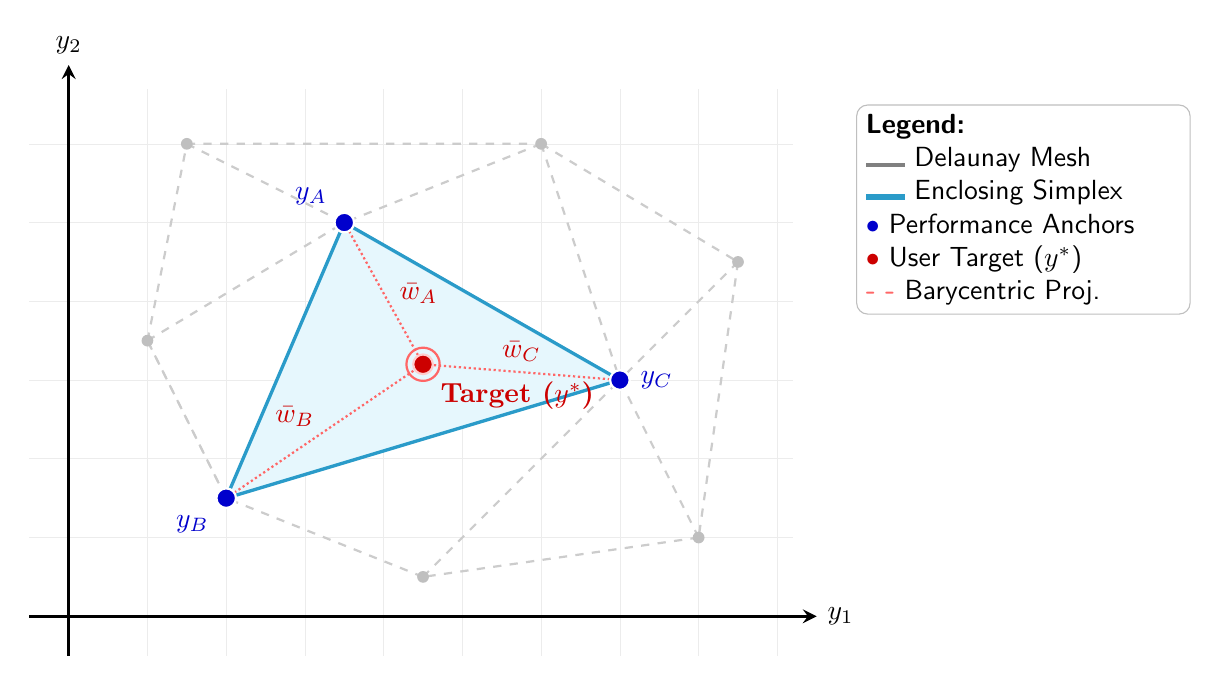
\begin{tikzpicture}[
    >=stealth,
    font=\sffamily,
    % Styles
    bg_point/.style={circle, fill=gray!50, inner sep=1.5pt},
    anchor_point/.style={circle, fill=blue!80!black, inner sep=2.5pt, draw=white, thick},
    target_point/.style={circle, fill=red!80!black, inner sep=2.5pt, draw=red!20, thick},
    mesh_line/.style={gray!40, thick, dashed},
    active_edge/.style={cyan!80!black, very thick},
    bary_line/.style={red!60, thick, densely dotted}
]

    % ==========================================
    % 1. BACKGROUND GRID (Enhancement)
    % ==========================================
    % Adds a subtle mathematical coordinate feel to the Objective Space
    \draw[step=1cm, gray!15, very thin] (-0.5, -0.5) grid (9.2, 6.7);

    % ==========================================
    % 2. AXES
    % ==========================================
    \draw[->, very thick] (-0.5, 0) -- (9.5, 0) node[right, align=center] {$y_1$};
    \draw[->, very thick] (0, -0.5) -- (0, 7.0) node[above, align=center] {$y_2$};

    % ==========================================
    % 3. COORDINATES DEFINITION
    % ==========================================
    % The Active Simplex (Anchors)
    \coordinate (yA) at (3.5, 5.0);
    \coordinate (yB) at (2.0, 1.5);
    \coordinate (yC) at (7.0, 3.0);
    
    % The User Target
    \coordinate (target) at (4.5, 3.2);

    % Background Dataset Points
    \coordinate (p1) at (1.0, 3.5);
    \coordinate (p2) at (1.5, 6.0);
    \coordinate (p3) at (6.0, 6.0);
    \coordinate (p4) at (8.5, 4.5);
    \coordinate (p5) at (8.0, 1.0);
    \coordinate (p6) at (4.5, 0.5);

    % ==========================================
    % 4. BACKGROUND DELAUNAY MESH
    % ==========================================
    % Draw connections to form a triangulation
    \draw[mesh_line] (p1) -- (yA) (p1) -- (yB) (p1) -- (p2);
    \draw[mesh_line] (p2) -- (yA) (p2) -- (p3);
    \draw[mesh_line] (p3) -- (yA) (p3) -- (yC) (p3) -- (p4);
    \draw[mesh_line] (p4) -- (yC) (p4) -- (p5);
    \draw[mesh_line] (p5) -- (yC) (p5) -- (p6);
    \draw[mesh_line] (p6) -- (yC) (p6) -- (yB);
    \draw[mesh_line] (yB) -- (p1);

    % ==========================================
    % 5. ACTIVE SIMPLEX (The located triangle)
    % ==========================================
    % Fill and draw the specific triangle containing the target
    \filldraw[fill=cyan!10, draw=cyan!80!black, very thick, line join=round] 
        (yA) -- (yB) -- (yC) -- cycle;

    % ==========================================
    % 6. BARYCENTRIC WEIGHT INDICATORS
    % ==========================================
    % Lines from vertices to the target point to visualize barycentric coordinates
    \draw[bary_line] (yA) -- (target) node[midway, right, text=red!80!black, xshift=2pt] {\textbf{$\bar{w}_A$}};
    \draw[bary_line] (yB) -- (target) node[midway, above left, text=red!80!black, yshift=-2pt] {\textbf{$\bar{w}_B$}};
    \draw[bary_line] (yC) -- (target) node[midway, above, text=red!80!black] {\textbf{$\bar{w}_C$}};

    % ==========================================
    % 7. DRAW POINTS & LABELS (Drawn last to stay on top)
    % ==========================================
    % Background Points
    \foreach \p in {p1, p2, p3, p4, p5, p6} {
        \node[bg_point] at (\p) {};
    }

    % Anchors
    \node[anchor_point, label={[text=blue!80!black, font=\bfseries]above left:$y_A$}] at (yA) {};
    \node[anchor_point, label={[text=blue!80!black, font=\bfseries]below left:$y_B$}] at (yB) {};
    \node[anchor_point, label={[text=blue!80!black, font=\bfseries]right:$y_C$}] at (yC) {};

    % User Target Point
    % Draw a halo ring around it to make it pop
    \draw[red!60, thick] (target) circle (6pt);
    \node[target_point, label={[text=red!80!black, font=\bfseries]below right:Target ($y^*$)}] at (target) {};

    % ==========================================
    % 8. LEGEND / ANNOTATION BOX (Shifted completely to the right)
    % ==========================================
    % Anchored north west at x=10.0 so it never overlaps the plot
    \node[draw=gray!50, fill=white, rounded corners, text width=4cm, align=left, anchor=north west] 
        at (10.0, 6.5) {
        \textbf{Legend:}\\
        \textcolor{gray}{\rule{0.5cm}{1.5pt}} Delaunay Mesh\\
        \textcolor{cyan!80!black}{\rule{0.5cm}{2pt}} Enclosing Simplex\\
        \textcolor{blue!80!black}{$\bullet$} Performance Anchors\\
        \textcolor{red!80!black}{$\bullet$} User Target ($y^*$)\\
        \textcolor{red!60}{\textbf{- -}} Barycentric Proj.
    };

\end{tikzpicture}